\setchapterstyle{kao}

\setchapterimage[6cm]{gid-3-org}
\setchapterpreamble[u]{\margintoc}

\chapter{Metodolog\'ia de Revisi\'on Documental }
\label{ch:met-RevDoc}
\index{revisi\'on documental!metodolg\'ia}

       En esta parte se presenta la metodología para la revisión documental. La metodología se presenta en dos fases :  \index{metodolog\'ia!dise\~no de la b\'usqueda}
		\index{metodolog\'ia!an\'alisis cr\'itico}

\begin{itemize}
	\item Diseño de la Búsqueda. Esta fase es la que se detalla en este cap\'itulo. Consta de los siguientes pasos:  
	\begin{description}
		\item Definición de Descriptores
		\item Uso de Tesauros
		\item Estrategias de búsquedas
		\item Diseño de la búsqueda
		\item Bases de Datos para la búsqueda
	\end{description}
	\item Análisis Crítico de Documentos. En esta fase se completa la metodolog\'ia de revisi\'on documental
	\begin{description}
		\item Organización de la información acopiada
		\item Criterio de selección de documentos
		\item Resultados de la búsqueda
	\end{description}
\end{itemize} 

\begin{marginfigure}[-3cm]%
	\includegraphics[width=\linewidth]{imagen1}
	%	\caption{Fichas bibliogr\'aficas }
	%	\label{fig:Fichas}
\end{marginfigure} 

Ejemplificaremos la metodología mediante el planteamiento de dos pesquisas. La primera pregunta de  investigación planteada en  \sidecite{Naranjo2010}:
 ?` Los Sistemas de Información Documental, en tanto medios, cómo posibilitarían la estructuración de los datos y la información en conocimiento con fines formativos en la educación superior ?

La segunda es una investigación dirigida a conocer  como evaluar recursos de internet "necesidad de evaluación de los recursos de Internet"; "Preocupación del bibliotecario por los recursos de evaluación"; y "Criterios para evaluar diferentes recursos de Internet",  que se presenta en  \sidecite{Kaushik2012}.

\section{ Definición de Descriptores}

\index{b\'usqueda de informaci\'on!tesauro} 

  Los descriptores o palabras claves  establecen un vocabulario controlado o los temas que  trata  un texto. En una pregunta o preguntas de investigación, definen las áreas de conocimientos  que se deben explorar para un búsqueda de documentos.
  
  En la pregunta de investigación que se usan como ejemplo para ilustrar este concepto: 
  
  \begin{marginfigure}[-3.3cm]%
  	\includegraphics[width=\linewidth]{KeyW}
  	%	\caption{Fichas bibliogr\'aficas }
  	%	\label{fig:Fichas}
  \end{marginfigure}
  
  
   ?` Los Sistemas de Información Documental, en tanto medios, cómo posibilitarían la estructuración de los datos y la información en conocimiento con fines formativos en la educación superior?    
  se infiere que los descriptores son los siguientes: 
  
  \begin{marginfigure}[-3cm]%
  	\includegraphics[width=\linewidth]{keyW}
  	%	\caption{Fichas bibliogr\'aficas }
  	%	\label{fig:Fichas}
  \end{marginfigure}
  
  	\marginnote[-4.2cm]{
  	\begin{kaobox}[frametitle= Palabras de b\'usqueda ]
  		\begin{description}
  			\item[Sistema de información \\ documental] 
  			\item[Dato] 
  			\item[Información] 
  			\item[Conocimiento] 
  			\item[Sistema didáctico] 
  			\item[Información] 
  			\item[Estrategia didáctica] 
  		\end{description}
  		
  	\end{kaobox}
  } 
  
 
  En la  investigación dirigida a conocer a conocer como evaluar recursos de internet "necesidad de evaluación de los recursos de Internet"; "Preocupación del bibliotecario por los recursos de evaluación"; y "Criterios para evaluar diferentes recursos de Internet", las palabras de  búsquedas son:
   
   	\marginnote[-2.2cm]{
   	\begin{kaobox}[frametitle= Palabras de b\'usqueda]
   		\begin{description}
   			\item[recursos de internet] 
   			\item[evaluar] 
   			\item[criterios de evaluación] 
   			\item[bibliotecario]  
   		\end{description}
   		
   	\end{kaobox}
   } 
   
    \begin{kaobox}[frametitle=Ejercicio]
    	Establezca una pregunta o preguntas de investigación que direccionen una revisión bibliográfica. Defina las palabras claves.
    \end{kaobox}

\begin{marginfigure}[-1.2cm]%
	\includegraphics[width=\linewidth]{pregunta}
	%	\caption{Fichas bibliogr\'aficas }
	%	\label{fig:Fichas}
\end{marginfigure}

\section{Consulta de tesauro}

El propósito de consultar un tesauro es conocer, además de la definición del término, los sinónimos, antónimos y la jerarquía de palabras o palabras derivadas del término buscado.

\index{b\'usqueda de informaci\'on!tesauro}
 
 
 	\marginnote[-3.2cm]{
	\begin{kaobox}[frametitle= Tesauro]

		El Tesauro  es una lista controlada y estructurada de términos para el análisis temático y la búsqueda de documentos y publicaciones en los campos de la educación, cultura, ciencias naturales, ciencias sociales y humanas, comunicación e información  
			
	\end{kaobox}
} 

Una busqueda del t\'ermino \textins{tesauros en l\'inea} con su buscador en la red, le muestra un conjunto de tesauros disponibles que puede usar. 
\index{b\'usqueda de informaci\'on!tesauro en l\'inea}


	\marginnote {
	\begin{kaobox}[frametitle= Tesauros en Finanzas]	
			En este enlace puede consultar el tesuaro  del \'area de  	\href{http://vocabularies.unesco.org/browser/thesaurus/es/page/concept663}{Tesauro de finanzas}  
		
 
	\end{kaobox}
} 

La consulta en tesauros (por ejemplo, usaremos el tesauro de la UNESCO) acerca de palabras relacionadas a las palabras claves, arrojan solo sinónimos para el primer término, en la consulta de \sidecite{Naranjo2010}: 



\begin{description}
	\item[Sistema de información documental] servicio bibliográfico, biblioteca
	\item [Dato]
	\item [Información]
	\item [Conocimiento]
	\item [Sistema didáctico]
	\item [Estrategia didáctica ]
\end{description}


Para la investigación establecida por \sidecite{Kaushik2012}: 


\begin{description}
	\item [recursos de internet:]  fuentes de internet
	\item [evaluación:]  medición
	\item [criterios de evaluación]
	\item [bibliotecario ]
\end{description}

 

Ademas de las palabras relacionadas, los conceptos plasmados en el tesauro se incluyen  en el documento cuando define el problema de su investigación  o el área de su estudio.

\begin{marginfigure}[1.2cm]%
	\includegraphics[width=\linewidth]{pregunta}
	%	\caption{Fichas bibliogr\'aficas }
	%	\label{fig:Fichas}
\end{marginfigure}
\section{Establecer las estrategias de búsquedas}

 \begin{kaobox}[frametitle= Ejercicio ]
Explore la internet usando su buscador de preferencia, explore los tesauros disponibles. Elija los que va a usar como fuente de información y busque las palabras relacionadas y los conceptos concernientes a las palabras claves de su investigación. Use Zotero o el gestor de documento preferido para capturar esas fuentes de datos. Indique en su respuesta: Tesauro usado en formato de normas APA. Si usa el gestor de documento, solo cópielo de se bibliografía. Resultado de las consultas en el tesauro: palabras relacionadas y conceptos asociados a las palabras claves  	
 \end{kaobox}


\begin{marginfigure}[-2cm]
	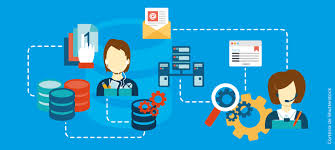
\includegraphics[width=\linewidth]{criterio}
	%	\caption{Fichas bibliogr\'aficas }
	%	\label{fig:Fichas}
\end{marginfigure}

Se arman las búsquedas en la biblioteca estableciendo las cadenas de búsquedas. La estrategia para armar estas cadenas es combinar las palabras claves usando los conectores booleanos or, and, not. 
  
Las cadenas de búsquedas van a ser usadas como entrada en los buscadores de documentos. Note las asociaciones de las claves expresadas por medio de paréntesis. 
Por ejemplo:
(Sistema de información documental \textbf{or} servicio bibliográfico \textbf{or} biblioteca )  se agruparon de esta manera ya que son términos homónimos.
((dato) \textbf{or} (información) \textbf{or} (conocimiento) )  a pesar de tener distintas acepciones,  se buscarán documentos que tengan cualquiera de esas palabras

\begin{marginfigure}[-2.2cm]
	\includegraphics[width=\linewidth]{imagen3}
	%	\caption{Fichas bibliogr\'aficas }
	%	\label{fig:Fichas}
\end{marginfigure}

Las cadenas establecidas son:
\begin{itemize}
	\item (Sistema de información documental \textbf{or} servicio bibliográfico \textbf{or} biblioteca) \textbf{and} ((dato) \textbf{or} (información) \textbf{or} (conocimiento) ) \textbf{or} (Sistema didáctico ) \textbf{or}  (Estrategia didáctica)
	
	\item (Sistema de información documental \textbf{or} servicio bibliográfico \textbf{or} biblioteca) \textbf{and} (Sistema didáctico ) \textbf{not} (Estrategia didáctica) \textbf{or} ((dato) \textbf{or} (información) \textbf{or} (conocimiento) ) 
	
	\item (Sistema de información documental \textbf{or} servicio bibliográfico \textbf{or} biblioteca) \textbf{and} (Estrategia didáctica) \textbf{not} (Sistema didáctico )  \textbf{or} ((dato) \textbf{or} (información) \textbf{or} (conocimiento) ) 
\end{itemize}

 \begin{marginfigure}[-1.2cm]%
 	\includegraphics[width=\linewidth]{pregunta}
 	%	\caption{Fichas bibliogr\'aficas }
 	%	\label{fig:Fichas}
 \end{marginfigure}

\begin{kaobox}[frametitle= Ejercicio]
Indique las cuales serían las cadenas de búsqueda que usaría para su recolección de investigación. 	
\end{kaobox}


 
 \section{Base de Datos para la búsqueda}

\index{b\'usqueda de informaci\'on!base de datos}                 
 La búsqueda de la literatura para elaborar un artículo de revisión se puede realizar en varios tipos de fuentes de información. Existen diferentes clasificaciones de los tipos de documentos que podemos manejar en nuestra búsqueda bibliográfica. \sidecite{Paiva2007}
 Una de las más utilizadas es aquella que distingue entre tipos de documentos provenientes de:
 

 
 \begin{description}  
 	\index{b\'usqueda de informaci\'on!fuentes }
 	\item[Fuentes primarias.] Originales, transmiten información directa (artículos originales, tesis).
 	
 	\item[Fuentes secundarias.] Ofrecen descripciones de los documentos primarios (catálogos, bases de datos, revisiones sistemáticas, resúmenes). 
 	
 	\item[Fuentes Terciarias.] Sintetizan los documentos primarios y los secundarios (directorios).
 \end{description}
 
 Las bases de datos son una fuente secundaria de datos homogéneos recuperables a través de internet. Contienen registros o referencias bibliográficas completas de fuentes primarias (artículos de investigación, libros, tesis, entre otros), organizados en campos que cubren todos los aspectos de la información (título, autor, resumen, etc.)
 
  \begin{marginfigure}[-2cm]%
 	\includegraphics[width=\linewidth]{basedatos}
 	%	\caption{Fichas bibliogr\'aficas }
 	%	\label{fig:Fichas}
 \end{marginfigure}
 
 Establecer las bases de datos especializadas donde se van a extraer información. Ejemplos de estas bases de datos:
 
 \begin{marginfigure}[2cm]%
 	\includegraphics[width=\linewidth]{imagen2}
 	%	\caption{Fichas bibliogr\'aficas }
 	%	\label{fig:Fichas}
 \end{marginfigure}
 
 \begin{itemize}
 	\item  \href{https://www.ebsco.com/es/productos/bases-de-datos}{LISTA}: Library, Information Science \& Technology Abstracts. 
 	
 	\item \href{https://about.proquest.com/products-services/lisa-set-c.html}{LISA}: Library and Information Science Abstract.  
 	
 	\item  \href{https://libguides.du.edu/c.php?g=90436&p=582594}{ERICH}: Education Resources Information Center, H. W. Wilson and Emerald.   
 	 
 	\item   Motor de búsqueda \textbf{Google}, \textbf{Google Scholar},\textbf{CiteseerX}, \textbf{Science Direct}.
 	
  	\item  	Redalyc: Red de Revistas Científicas de América Latina y el Caribe
 \end{itemize}
   
 
 Las bases de datos seleccionadas para la búsqueda pueden presentarse en una tabla que sintetice esta colección. La estructura del cuadro \ref{tab:recursos} es la siguiente. Cada celda contiene información de un recurso:
 
  	\begin{table}[h] 
  	\footnotesize%
  	\begin{center}
  		\footnotesize
  		\begin{tabular}{|c|c|c|c|}
  			\hline
    		   Recurso &   \multicolumn{3}{|c|}{Nombres}  \\
  			\hline  			
  			\tiny{Bibliotecas Universitarias} &   &  &  \\
  				\hline  			
  		\tiny{Sitios Web} & \tiny{Google}  & \tiny{CieseerX} & \\
  			\hline  			
  		\tiny{Bases de Datos}  &  \tiny{Redalyc} &  & \\
  			\hline  			
  		\tiny{Revistas Electr\'onicas} &  \tiny{Strategos} & & \\
  			\hline  	  		
  		\end{tabular}
  	\end{center}
  	\caption{Recursos y Sistemas de Información }
  	\label{tab:recursos}
  \end{table}
  
 
  \begin{marginfigure}[1.2cm]%
 	\includegraphics[width=\linewidth]{pregunta}
 	%	\caption{Fichas bibliogr\'aficas }
 	%	\label{fig:Fichas}
 \end{marginfigure}
 
 
 \begin{kaobox} [frametitle= Ejercicio ]
 	Los artículos de revisión documental o estado del arte se basan en documentos provenientes de fuentes primarias. Indique cuales serían las bases de datos para la búsqueda de estos documentos.
 	Presente esas bases de datos en la tabla de Recursos y Sistemas de Información.
 	
 	\end{kaobox}
 

 
  
     



